\documentclass[twoside]{book}

% Packages required by doxygen
\usepackage{fixltx2e}
\usepackage{calc}
\usepackage{doxygen}
\usepackage[export]{adjustbox} % also loads graphicx
\usepackage{graphicx}
\usepackage[utf8]{inputenc}
\usepackage{makeidx}
\usepackage{multicol}
\usepackage{multirow}
\PassOptionsToPackage{warn}{textcomp}
\usepackage{textcomp}
\usepackage[nointegrals]{wasysym}
\usepackage[table]{xcolor}

% NLS support packages
\usepackage[spanish]{babel}
% Font selection
\usepackage[T1]{fontenc}
\usepackage[scaled=.90]{helvet}
\usepackage{courier}
\usepackage{amssymb}
\usepackage{sectsty}
\renewcommand{\familydefault}{\sfdefault}
\allsectionsfont{%
  \fontseries{bc}\selectfont%
  \color{darkgray}%
}
\renewcommand{\DoxyLabelFont}{%
  \fontseries{bc}\selectfont%
  \color{darkgray}%
}
\newcommand{\+}{\discretionary{\mbox{\scriptsize$\hookleftarrow$}}{}{}}

% Page & text layout
\usepackage{geometry}
\geometry{%
  a4paper,%
  top=2.5cm,%
  bottom=2.5cm,%
  left=2.5cm,%
  right=2.5cm%
}
\tolerance=750
\hfuzz=15pt
\hbadness=750
\setlength{\emergencystretch}{15pt}
\setlength{\parindent}{0cm}
\setlength{\parskip}{3ex plus 2ex minus 2ex}
\makeatletter
\renewcommand{\paragraph}{%
  \@startsection{paragraph}{4}{0ex}{-1.0ex}{1.0ex}{%
    \normalfont\normalsize\bfseries\SS@parafont%
  }%
}
\renewcommand{\subparagraph}{%
  \@startsection{subparagraph}{5}{0ex}{-1.0ex}{1.0ex}{%
    \normalfont\normalsize\bfseries\SS@subparafont%
  }%
}
\makeatother

% Headers & footers
\usepackage{fancyhdr}
\pagestyle{fancyplain}
\fancyhead[LE]{\fancyplain{}{\bfseries\thepage}}
\fancyhead[CE]{\fancyplain{}{}}
\fancyhead[RE]{\fancyplain{}{\bfseries\leftmark}}
\fancyhead[LO]{\fancyplain{}{\bfseries\rightmark}}
\fancyhead[CO]{\fancyplain{}{}}
\fancyhead[RO]{\fancyplain{}{\bfseries\thepage}}
\fancyfoot[LE]{\fancyplain{}{}}
\fancyfoot[CE]{\fancyplain{}{}}
\fancyfoot[RE]{\fancyplain{}{\bfseries\scriptsize Generado por Doxygen }}
\fancyfoot[LO]{\fancyplain{}{\bfseries\scriptsize Generado por Doxygen }}
\fancyfoot[CO]{\fancyplain{}{}}
\fancyfoot[RO]{\fancyplain{}{}}
\renewcommand{\footrulewidth}{0.4pt}
\renewcommand{\chaptermark}[1]{%
  \markboth{#1}{}%
}
\renewcommand{\sectionmark}[1]{%
  \markright{\thesection\ #1}%
}

% Indices & bibliography
\usepackage{natbib}
\usepackage[titles]{tocloft}
\setcounter{tocdepth}{3}
\setcounter{secnumdepth}{5}
\makeindex

% Hyperlinks (required, but should be loaded last)
\usepackage{ifpdf}
\ifpdf
  \usepackage[pdftex,pagebackref=true]{hyperref}
\else
  \usepackage[ps2pdf,pagebackref=true]{hyperref}
\fi
\hypersetup{%
  colorlinks=true,%
  linkcolor=blue,%
  citecolor=blue,%
  unicode%
}

% Custom commands
\newcommand{\clearemptydoublepage}{%
  \newpage{\pagestyle{empty}\cleardoublepage}%
}

\usepackage{caption}
\captionsetup{labelsep=space,justification=centering,font={bf},singlelinecheck=off,skip=4pt,position=top}

%===== C O N T E N T S =====

\begin{document}

% Titlepage & ToC
\hypersetup{pageanchor=false,
             bookmarksnumbered=true,
             pdfencoding=unicode
            }
\pagenumbering{roman}
\begin{titlepage}
\vspace*{7cm}
\begin{center}%
{\Large Letras }\\
\vspace*{1cm}
{\large Generado por Doxygen 1.8.11}\\
\end{center}
\end{titlepage}
\clearemptydoublepage
\tableofcontents
\clearemptydoublepage
\pagenumbering{arabic}
\hypersetup{pageanchor=true}

%--- Begin generated contents ---
\chapter{Índice de clases}
\section{Lista de clases}
Lista de las clases, estructuras, uniones e interfaces con una breve descripción\+:\begin{DoxyCompactList}
\item\contentsline{section}{\hyperlink{class_arbol_general}{Arbol\+General$<$ Tbase $>$} }{\pageref{class_arbol_general}}{}
\item\contentsline{section}{\hyperlink{class_bolsa_letras}{Bolsa\+Letras} \\*T\+DA \hyperlink{class_bolsa_letras}{Bolsa\+Letras} {\bfseries Definición\+:} \hyperlink{class_bolsa_letras}{Bolsa\+Letras} guarda todos los caracteres que se pueden usar y obtiene las letras disponibles en el juego de forma aleatoria }{\pageref{class_bolsa_letras}}{}
\item\contentsline{section}{\hyperlink{class_conjunto_letras}{Conjunto\+Letras} \\*T\+DA \hyperlink{_conjunto_letras_8h}{Conjunto\+Letras.\+h} {\bfseries Definición\+:} La clase conjunto letras guarda un conjunto de Letras }{\pageref{class_conjunto_letras}}{}
\item\contentsline{section}{\hyperlink{class_arbol_general_1_1const__iter__preorden}{Arbol\+General$<$ Tbase $>$\+::const\+\_\+iter\+\_\+preorden} }{\pageref{class_arbol_general_1_1const__iter__preorden}}{}
\item\contentsline{section}{\hyperlink{class_diccionario}{Diccionario} \\*Clase \hyperlink{class_diccionario}{Diccionario} {\bfseries Definición\+:} La clase diccionario contiene un arbol general en el que se guardan las letras formando palabras }{\pageref{class_diccionario}}{}
\item\contentsline{section}{\hyperlink{class_arbol_general_1_1iter__preorden}{Arbol\+General$<$ Tbase $>$\+::iter\+\_\+preorden} }{\pageref{class_arbol_general_1_1iter__preorden}}{}
\item\contentsline{section}{\hyperlink{class_diccionario_1_1iterator}{Diccionario\+::iterator} \\*Iterador del diccionario }{\pageref{class_diccionario_1_1iterator}}{}
\item\contentsline{section}{\hyperlink{class_letra}{Letra} \\*T\+DA \hyperlink{class_letra}{Letra} {\bfseries Definición\+:} La clase letra guarda la informacion sobre cada letra }{\pageref{class_letra}}{}
\end{DoxyCompactList}

\chapter{Indice de archivos}
\section{Lista de archivos}
Lista de todos los archivos documentados y con descripciones breves\+:\begin{DoxyCompactList}
\item\contentsline{section}{inc/{\bfseries Arbol\+General.\+h} }{\pageref{_arbol_general_8h}}{}
\item\contentsline{section}{inc/\hyperlink{_bolsa_letras_8h}{Bolsa\+Letras.\+h} }{\pageref{_bolsa_letras_8h}}{}
\item\contentsline{section}{inc/\hyperlink{_conjunto_letras_8h}{Conjunto\+Letras.\+h} }{\pageref{_conjunto_letras_8h}}{}
\item\contentsline{section}{inc/\hyperlink{diccionario_8h}{diccionario.\+h} }{\pageref{diccionario_8h}}{}
\item\contentsline{section}{inc/\hyperlink{_letra_8h}{Letra.\+h} }{\pageref{_letra_8h}}{}
\end{DoxyCompactList}

\chapter{Documentación de las clases}
\hypertarget{class_arbol_general}{}\section{Referencia de la plantilla de la Clase Arbol\+General$<$ Tbase $>$}
\label{class_arbol_general}\index{Arbol\+General$<$ Tbase $>$@{Arbol\+General$<$ Tbase $>$}}
\subsection*{Clases}
\begin{DoxyCompactItemize}
\item 
class \hyperlink{class_arbol_general_1_1const__iter__preorden}{const\+\_\+iter\+\_\+preorden}
\item 
class \hyperlink{class_arbol_general_1_1iter__preorden}{iter\+\_\+preorden}
\end{DoxyCompactItemize}
\subsection*{Tipos públicos}
\begin{DoxyCompactItemize}
\item 
typedef struct nodo $\ast$ {\bfseries Nodo}\hypertarget{class_arbol_general_a12cc1b74a9095d89bc7334290d332f7a}{}\label{class_arbol_general_a12cc1b74a9095d89bc7334290d332f7a}

\end{DoxyCompactItemize}
\subsection*{Métodos públicos}
\begin{DoxyCompactItemize}
\item 
{\bfseries Arbol\+General} (const Tbase \&e)\hypertarget{class_arbol_general_a8ddac1a024f05bee96f4c259fad76c4c}{}\label{class_arbol_general_a8ddac1a024f05bee96f4c259fad76c4c}

\item 
{\bfseries Arbol\+General} (const \hyperlink{class_arbol_general}{Arbol\+General}$<$ Tbase $>$ \&v)\hypertarget{class_arbol_general_ad7926f03eb051b9691d57f4e508cad4d}{}\label{class_arbol_general_ad7926f03eb051b9691d57f4e508cad4d}

\item 
\hyperlink{class_arbol_general}{Arbol\+General}$<$ Tbase $>$ \& {\bfseries operator=} (const \hyperlink{class_arbol_general}{Arbol\+General}$<$ Tbase $>$ \&v)\hypertarget{class_arbol_general_aebd3723e9929b905445127a754a26759}{}\label{class_arbol_general_aebd3723e9929b905445127a754a26759}

\item 
void {\bfseries Asigna\+Raiz} (const Tbase \&e)\hypertarget{class_arbol_general_a84781986cd57390540600494303b0e9d}{}\label{class_arbol_general_a84781986cd57390540600494303b0e9d}

\item 
Nodo {\bfseries raiz} () const \hypertarget{class_arbol_general_a385099b0c15ac15cf15a954725e1e8a2}{}\label{class_arbol_general_a385099b0c15ac15cf15a954725e1e8a2}

\item 
Nodo {\bfseries hijomasizquierda} (const Nodo n) const \hypertarget{class_arbol_general_aebf8b37c050c73a9bff1f697efd931b5}{}\label{class_arbol_general_aebf8b37c050c73a9bff1f697efd931b5}

\item 
Nodo {\bfseries hermanoderecha} (const Nodo n) const \hypertarget{class_arbol_general_a854ad15f86991fdc0e2257b3d32a98b8}{}\label{class_arbol_general_a854ad15f86991fdc0e2257b3d32a98b8}

\item 
Nodo {\bfseries padre} (const Nodo n) const \hypertarget{class_arbol_general_a9027dd4b060e1216241d4cfe9f2898e7}{}\label{class_arbol_general_a9027dd4b060e1216241d4cfe9f2898e7}

\item 
Tbase \& {\bfseries etiqueta} (const Nodo n)\hypertarget{class_arbol_general_ac08063e5bcc034ab723d21c0fea44b46}{}\label{class_arbol_general_ac08063e5bcc034ab723d21c0fea44b46}

\item 
const Tbase \& {\bfseries etiqueta} (const Nodo n) const \hypertarget{class_arbol_general_a191b525e0e6c8dec3a1430139f516847}{}\label{class_arbol_general_a191b525e0e6c8dec3a1430139f516847}

\item 
void {\bfseries asignar\+\_\+subarbol} (const \hyperlink{class_arbol_general}{Arbol\+General}$<$ Tbase $>$ \&orig, const Nodo nod)\hypertarget{class_arbol_general_ad9fddc80b179cac8eddc113a048334c1}{}\label{class_arbol_general_ad9fddc80b179cac8eddc113a048334c1}

\item 
void {\bfseries podar\+\_\+hijomasizquierda} (Nodo n, \hyperlink{class_arbol_general}{Arbol\+General}$<$ Tbase $>$ \&dest)\hypertarget{class_arbol_general_a7f2fa2d9be4af4b7be1c334819a04c39}{}\label{class_arbol_general_a7f2fa2d9be4af4b7be1c334819a04c39}

\item 
void {\bfseries podar\+\_\+hermanoderecha} (Nodo n, \hyperlink{class_arbol_general}{Arbol\+General}$<$ Tbase $>$ \&dest)\hypertarget{class_arbol_general_a81282ccc37494f1e13042e06ea475fb6}{}\label{class_arbol_general_a81282ccc37494f1e13042e06ea475fb6}

\item 
void {\bfseries insertar\+\_\+hijomasizquierda} (Nodo n, \hyperlink{class_arbol_general}{Arbol\+General}$<$ Tbase $>$ \&rama)\hypertarget{class_arbol_general_acf95226edb2a4e4c7fba82aaa82d0ec9}{}\label{class_arbol_general_acf95226edb2a4e4c7fba82aaa82d0ec9}

\item 
void {\bfseries insertar\+\_\+hermanoderecha} (Nodo n, \hyperlink{class_arbol_general}{Arbol\+General}$<$ Tbase $>$ \&rama)\hypertarget{class_arbol_general_a855d44f14a9ef638f8dd46376fc2f961}{}\label{class_arbol_general_a855d44f14a9ef638f8dd46376fc2f961}

\item 
void {\bfseries clear} ()\hypertarget{class_arbol_general_a3ae21db42586b23ccc082aeb321db56f}{}\label{class_arbol_general_a3ae21db42586b23ccc082aeb321db56f}

\item 
int {\bfseries size} () const \hypertarget{class_arbol_general_a69a2c10bedbf77dbc23baea0a731a02d}{}\label{class_arbol_general_a69a2c10bedbf77dbc23baea0a731a02d}

\item 
bool {\bfseries empty} () const \hypertarget{class_arbol_general_ab7b59c8fe7e74f78f3533965460a6c9a}{}\label{class_arbol_general_ab7b59c8fe7e74f78f3533965460a6c9a}

\item 
bool {\bfseries operator==} (const \hyperlink{class_arbol_general}{Arbol\+General}$<$ Tbase $>$ \&v) const \hypertarget{class_arbol_general_a5c7db1c3f26d29b887ba906d02397a8d}{}\label{class_arbol_general_a5c7db1c3f26d29b887ba906d02397a8d}

\item 
bool {\bfseries operator!=} (const \hyperlink{class_arbol_general}{Arbol\+General}$<$ Tbase $>$ \&v) const \hypertarget{class_arbol_general_ab5b783cb068a394511f99e08a827cdda}{}\label{class_arbol_general_ab5b783cb068a394511f99e08a827cdda}

\item 
\hyperlink{class_arbol_general_1_1iter__preorden}{iter\+\_\+preorden} {\bfseries begin} ()\hypertarget{class_arbol_general_afbaa00d73656de3957e6f0427ba53347}{}\label{class_arbol_general_afbaa00d73656de3957e6f0427ba53347}

\item 
\hyperlink{class_arbol_general_1_1const__iter__preorden}{const\+\_\+iter\+\_\+preorden} {\bfseries begin} () const \hypertarget{class_arbol_general_a63912c2167da4335982ea59948404d4a}{}\label{class_arbol_general_a63912c2167da4335982ea59948404d4a}

\item 
\hyperlink{class_arbol_general_1_1iter__preorden}{iter\+\_\+preorden} {\bfseries end} ()\hypertarget{class_arbol_general_a7d6434353f5d55acf8c22226838da586}{}\label{class_arbol_general_a7d6434353f5d55acf8c22226838da586}

\item 
\hyperlink{class_arbol_general_1_1const__iter__preorden}{const\+\_\+iter\+\_\+preorden} {\bfseries end} () const \hypertarget{class_arbol_general_a457b326a6347bb4d9b1cf6a062b32988}{}\label{class_arbol_general_a457b326a6347bb4d9b1cf6a062b32988}

\end{DoxyCompactItemize}
\subsection*{Amigas}
\begin{DoxyCompactItemize}
\item 
{\footnotesize template$<$class T $>$ }\\std\+::istream \& {\bfseries operator$>$$>$} (std\+::istream \&in, \hyperlink{class_arbol_general}{Arbol\+General}$<$ T $>$ \&v)\hypertarget{class_arbol_general_ab1318141f030856da7dcfc1c7a162565}{}\label{class_arbol_general_ab1318141f030856da7dcfc1c7a162565}

\item 
{\footnotesize template$<$class T $>$ }\\std\+::ostream \& {\bfseries operator$<$$<$} (std\+::ostream \&out, const \hyperlink{class_arbol_general}{Arbol\+General}$<$ T $>$ \&v)\hypertarget{class_arbol_general_a4e1153e673608d812c48de2a33bbead0}{}\label{class_arbol_general_a4e1153e673608d812c48de2a33bbead0}

\end{DoxyCompactItemize}


La documentación para esta clase fue generada a partir del siguiente fichero\+:\begin{DoxyCompactItemize}
\item 
inc/Arbol\+General.\+h\end{DoxyCompactItemize}

\hypertarget{class_bolsa_letras}{}\section{Referencia de la Clase Bolsa\+Letras}
\label{class_bolsa_letras}\index{Bolsa\+Letras@{Bolsa\+Letras}}


T\+DA \hyperlink{class_bolsa_letras}{Bolsa\+Letras} {\bfseries Definición\+:} \hyperlink{class_bolsa_letras}{Bolsa\+Letras} guarda todos los caracteres que se pueden usar y obtiene las letras disponibles en el juego de forma aleatoria.  




{\ttfamily \#include $<$Bolsa\+Letras.\+h$>$}

\subsection*{Métodos públicos}
\begin{DoxyCompactItemize}
\item 
\hyperlink{class_bolsa_letras_a2e269014b3a51359195e7b288a4b37c6}{Bolsa\+Letras} ()\hypertarget{class_bolsa_letras_a2e269014b3a51359195e7b288a4b37c6}{}\label{class_bolsa_letras_a2e269014b3a51359195e7b288a4b37c6}

\begin{DoxyCompactList}\small\item\em Constructor sin argumentos de \hyperlink{class_bolsa_letras}{Bolsa\+Letras}. \end{DoxyCompactList}\item 
\hyperlink{class_bolsa_letras_af412cf1648cf99bbf0e6ac897cdf6794}{Bolsa\+Letras} (\hyperlink{class_conjunto_letras}{Conjunto\+Letras} c)
\begin{DoxyCompactList}\small\item\em Constructor con argumentos de \hyperlink{class_bolsa_letras}{Bolsa\+Letras}. \end{DoxyCompactList}\item 
void \hyperlink{class_bolsa_letras_ac77fda91eebd34ba9f5b880ffe4a538b}{elimina\+\_\+letra} (char letra)
\begin{DoxyCompactList}\small\item\em Elimina un caracter de dequerandom. \end{DoxyCompactList}\item 
deque$<$ char $>$ \hyperlink{class_bolsa_letras_a8f921efe87a007d196cbf48b9fe103e9}{Get\+Randomletras} (int n)
\begin{DoxyCompactList}\small\item\em Obtiene un numero n de letras aleatorias disponibles en el campo letras. \end{DoxyCompactList}\item 
\hyperlink{class_bolsa_letras}{Bolsa\+Letras} \hyperlink{class_bolsa_letras_aba6f48dfaecf7e5635774913753d692b}{operator=} (\hyperlink{class_bolsa_letras}{Bolsa\+Letras} \&otra\+\_\+bolsa)
\begin{DoxyCompactList}\small\item\em Operador de asignacion de \hyperlink{class_bolsa_letras}{Bolsa\+Letras}. \end{DoxyCompactList}\item 
bool \hyperlink{class_bolsa_letras_a1976f62338d5216fad074e0b0fc0d6df}{pertenece} (char letra)
\begin{DoxyCompactList}\small\item\em Comprueba si un caracter se encuentra en letras. \end{DoxyCompactList}\item 
bool \hyperlink{class_bolsa_letras_aec338cef188e60e5737de9c336ec55ed}{pertenecerandom} (char letra)
\begin{DoxyCompactList}\small\item\em Comprueba si un caracter se encuentra en dequerandom. \end{DoxyCompactList}\item 
deque$<$ char $>$ \hyperlink{class_bolsa_letras_a9c0e1bf5538d08550f2a0ffbdeea6f71}{Getdequerandom} ()\hypertarget{class_bolsa_letras_a9c0e1bf5538d08550f2a0ffbdeea6f71}{}\label{class_bolsa_letras_a9c0e1bf5538d08550f2a0ffbdeea6f71}

\begin{DoxyCompactList}\small\item\em Devuelve una copia de dequerandom. \end{DoxyCompactList}\end{DoxyCompactItemize}


\subsection{Descripción detallada}
T\+DA \hyperlink{class_bolsa_letras}{Bolsa\+Letras} {\bfseries Definición\+:} \hyperlink{class_bolsa_letras}{Bolsa\+Letras} guarda todos los caracteres que se pueden usar y obtiene las letras disponibles en el juego de forma aleatoria. 

\subsection{Documentación del constructor y destructor}
\index{Bolsa\+Letras@{Bolsa\+Letras}!Bolsa\+Letras@{Bolsa\+Letras}}
\index{Bolsa\+Letras@{Bolsa\+Letras}!Bolsa\+Letras@{Bolsa\+Letras}}
\subsubsection[{\texorpdfstring{Bolsa\+Letras(\+Conjunto\+Letras c)}{BolsaLetras(ConjuntoLetras c)}}]{\setlength{\rightskip}{0pt plus 5cm}Bolsa\+Letras\+::\+Bolsa\+Letras (
\begin{DoxyParamCaption}
\item[{{\bf Conjunto\+Letras}}]{c}
\end{DoxyParamCaption}
)}\hypertarget{class_bolsa_letras_af412cf1648cf99bbf0e6ac897cdf6794}{}\label{class_bolsa_letras_af412cf1648cf99bbf0e6ac897cdf6794}


Constructor con argumentos de \hyperlink{class_bolsa_letras}{Bolsa\+Letras}. 


\begin{DoxyParams}{Parámetros}
{\em c} & \hyperlink{class_conjunto_letras}{Conjunto\+Letras} a parir del cual se quieren extraer todos los caracteres \\
\hline
\end{DoxyParams}


\subsection{Documentación de las funciones miembro}
\index{Bolsa\+Letras@{Bolsa\+Letras}!elimina\+\_\+letra@{elimina\+\_\+letra}}
\index{elimina\+\_\+letra@{elimina\+\_\+letra}!Bolsa\+Letras@{Bolsa\+Letras}}
\subsubsection[{\texorpdfstring{elimina\+\_\+letra(char letra)}{elimina_letra(char letra)}}]{\setlength{\rightskip}{0pt plus 5cm}void Bolsa\+Letras\+::elimina\+\_\+letra (
\begin{DoxyParamCaption}
\item[{char}]{letra}
\end{DoxyParamCaption}
)}\hypertarget{class_bolsa_letras_ac77fda91eebd34ba9f5b880ffe4a538b}{}\label{class_bolsa_letras_ac77fda91eebd34ba9f5b880ffe4a538b}


Elimina un caracter de dequerandom. 


\begin{DoxyParams}{Parámetros}
{\em letra} & el caracter que se quiere eliminar \\
\hline
\end{DoxyParams}
\index{Bolsa\+Letras@{Bolsa\+Letras}!Get\+Randomletras@{Get\+Randomletras}}
\index{Get\+Randomletras@{Get\+Randomletras}!Bolsa\+Letras@{Bolsa\+Letras}}
\subsubsection[{\texorpdfstring{Get\+Randomletras(int n)}{GetRandomletras(int n)}}]{\setlength{\rightskip}{0pt plus 5cm}deque$<$char$>$ Bolsa\+Letras\+::\+Get\+Randomletras (
\begin{DoxyParamCaption}
\item[{int}]{n}
\end{DoxyParamCaption}
)}\hypertarget{class_bolsa_letras_a8f921efe87a007d196cbf48b9fe103e9}{}\label{class_bolsa_letras_a8f921efe87a007d196cbf48b9fe103e9}


Obtiene un numero n de letras aleatorias disponibles en el campo letras. 


\begin{DoxyParams}{Parámetros}
{\em n} & numero de letras que se quiere obtener \\
\hline
\end{DoxyParams}
\begin{DoxyReturn}{Devuelve}
un deque de char con las letras obtenidas aleatoriamente 
\end{DoxyReturn}
\index{Bolsa\+Letras@{Bolsa\+Letras}!operator=@{operator=}}
\index{operator=@{operator=}!Bolsa\+Letras@{Bolsa\+Letras}}
\subsubsection[{\texorpdfstring{operator=(\+Bolsa\+Letras \&otra\+\_\+bolsa)}{operator=(BolsaLetras &otra_bolsa)}}]{\setlength{\rightskip}{0pt plus 5cm}{\bf Bolsa\+Letras} Bolsa\+Letras\+::operator= (
\begin{DoxyParamCaption}
\item[{{\bf Bolsa\+Letras} \&}]{otra\+\_\+bolsa}
\end{DoxyParamCaption}
)}\hypertarget{class_bolsa_letras_aba6f48dfaecf7e5635774913753d692b}{}\label{class_bolsa_letras_aba6f48dfaecf7e5635774913753d692b}


Operador de asignacion de \hyperlink{class_bolsa_letras}{Bolsa\+Letras}. 


\begin{DoxyParams}{Parámetros}
{\em otra\+\_\+bolsa} & Bolsa de la que se quieren obtener los datos \\
\hline
\end{DoxyParams}
\index{Bolsa\+Letras@{Bolsa\+Letras}!pertenece@{pertenece}}
\index{pertenece@{pertenece}!Bolsa\+Letras@{Bolsa\+Letras}}
\subsubsection[{\texorpdfstring{pertenece(char letra)}{pertenece(char letra)}}]{\setlength{\rightskip}{0pt plus 5cm}bool Bolsa\+Letras\+::pertenece (
\begin{DoxyParamCaption}
\item[{char}]{letra}
\end{DoxyParamCaption}
)}\hypertarget{class_bolsa_letras_a1976f62338d5216fad074e0b0fc0d6df}{}\label{class_bolsa_letras_a1976f62338d5216fad074e0b0fc0d6df}


Comprueba si un caracter se encuentra en letras. 


\begin{DoxyParams}{Parámetros}
{\em letra} & char del caracter que se quiere buscar \\
\hline
\end{DoxyParams}
\begin{DoxyReturn}{Devuelve}
true si esta, false si no esta 
\end{DoxyReturn}
\index{Bolsa\+Letras@{Bolsa\+Letras}!pertenecerandom@{pertenecerandom}}
\index{pertenecerandom@{pertenecerandom}!Bolsa\+Letras@{Bolsa\+Letras}}
\subsubsection[{\texorpdfstring{pertenecerandom(char letra)}{pertenecerandom(char letra)}}]{\setlength{\rightskip}{0pt plus 5cm}bool Bolsa\+Letras\+::pertenecerandom (
\begin{DoxyParamCaption}
\item[{char}]{letra}
\end{DoxyParamCaption}
)}\hypertarget{class_bolsa_letras_aec338cef188e60e5737de9c336ec55ed}{}\label{class_bolsa_letras_aec338cef188e60e5737de9c336ec55ed}


Comprueba si un caracter se encuentra en dequerandom. 


\begin{DoxyParams}{Parámetros}
{\em letra} & char del caracter que se quiere buscar \\
\hline
\end{DoxyParams}
\begin{DoxyReturn}{Devuelve}
true si esta, false si no esta 
\end{DoxyReturn}


La documentación para esta clase fue generada a partir del siguiente fichero\+:\begin{DoxyCompactItemize}
\item 
inc/\hyperlink{_bolsa_letras_8h}{Bolsa\+Letras.\+h}\end{DoxyCompactItemize}

\hypertarget{class_conjunto_letras}{}\section{Referencia de la Clase Conjunto\+Letras}
\label{class_conjunto_letras}\index{Conjunto\+Letras@{Conjunto\+Letras}}


T\+DA \hyperlink{_conjunto_letras_8h}{Conjunto\+Letras.\+h} {\bfseries Definición\+:} La clase conjunto letras guarda un conjunto de Letras.  




{\ttfamily \#include $<$Conjunto\+Letras.\+h$>$}

\subsection*{Métodos públicos}
\begin{DoxyCompactItemize}
\item 
deque$<$ \hyperlink{class_letra}{Letra} $>$ {\bfseries Getletras} ()\hypertarget{class_conjunto_letras_a7c8bb085fb038255526752a6dcdcf422}{}\label{class_conjunto_letras_a7c8bb085fb038255526752a6dcdcf422}

\item 
int \hyperlink{class_conjunto_letras_ad4e5706a02bf4875569cb6e177ff5902}{Getpuntuacion} (string palabra)
\begin{DoxyCompactList}\small\item\em Obtiene la puntuacion de una palabra. \end{DoxyCompactList}\end{DoxyCompactItemize}
\subsection*{Amigas}
\begin{DoxyCompactItemize}
\item 
istream \& \hyperlink{class_conjunto_letras_af5ad9e43f9a723151641010c62c9e8c0}{operator$>$$>$} (istream \&is, \hyperlink{class_conjunto_letras}{Conjunto\+Letras} \&C)
\begin{DoxyCompactList}\small\item\em Lee de un flujo de entrada un diccionario. \end{DoxyCompactList}\item 
ostream \& \hyperlink{class_conjunto_letras_a2bf98947859e69ca0855fe70eb0343ff}{operator$<$$<$} (ostream \&os, \hyperlink{class_conjunto_letras}{Conjunto\+Letras} \&C)
\begin{DoxyCompactList}\small\item\em Escribe en un flujo de salida un diccionario. \end{DoxyCompactList}\end{DoxyCompactItemize}


\subsection{Descripción detallada}
T\+DA \hyperlink{_conjunto_letras_8h}{Conjunto\+Letras.\+h} {\bfseries Definición\+:} La clase conjunto letras guarda un conjunto de Letras. 

\subsection{Documentación de las funciones miembro}
\index{Conjunto\+Letras@{Conjunto\+Letras}!Getpuntuacion@{Getpuntuacion}}
\index{Getpuntuacion@{Getpuntuacion}!Conjunto\+Letras@{Conjunto\+Letras}}
\subsubsection[{\texorpdfstring{Getpuntuacion(string palabra)}{Getpuntuacion(string palabra)}}]{\setlength{\rightskip}{0pt plus 5cm}int Conjunto\+Letras\+::\+Getpuntuacion (
\begin{DoxyParamCaption}
\item[{string}]{palabra}
\end{DoxyParamCaption}
)}\hypertarget{class_conjunto_letras_ad4e5706a02bf4875569cb6e177ff5902}{}\label{class_conjunto_letras_ad4e5706a02bf4875569cb6e177ff5902}


Obtiene la puntuacion de una palabra. 


\begin{DoxyParams}{Parámetros}
{\em palabra} & string del cual se quiere saber la puntuacion total \\
\hline
\end{DoxyParams}
\begin{DoxyReturn}{Devuelve}
in int con la puntuacion total 
\end{DoxyReturn}


\subsection{Documentación de las funciones relacionadas y clases amigas}
\index{Conjunto\+Letras@{Conjunto\+Letras}!operator$<$$<$@{operator$<$$<$}}
\index{operator$<$$<$@{operator$<$$<$}!Conjunto\+Letras@{Conjunto\+Letras}}
\subsubsection[{\texorpdfstring{operator$<$$<$}{operator<<}}]{\setlength{\rightskip}{0pt plus 5cm}ostream\& operator$<$$<$ (
\begin{DoxyParamCaption}
\item[{ostream \&}]{os, }
\item[{{\bf Conjunto\+Letras} \&}]{C}
\end{DoxyParamCaption}
)\hspace{0.3cm}{\ttfamily [friend]}}\hypertarget{class_conjunto_letras_a2bf98947859e69ca0855fe70eb0343ff}{}\label{class_conjunto_letras_a2bf98947859e69ca0855fe70eb0343ff}


Escribe en un flujo de salida un diccionario. 


\begin{DoxyParams}{Parámetros}
{\em os\+:flujo} & de salida \\
\hline
{\em D} & el objeto diccionario que se escribe \\
\hline
\end{DoxyParams}
\begin{DoxyReturn}{Devuelve}
el flujo de salida 
\end{DoxyReturn}
\index{Conjunto\+Letras@{Conjunto\+Letras}!operator$>$$>$@{operator$>$$>$}}
\index{operator$>$$>$@{operator$>$$>$}!Conjunto\+Letras@{Conjunto\+Letras}}
\subsubsection[{\texorpdfstring{operator$>$$>$}{operator>>}}]{\setlength{\rightskip}{0pt plus 5cm}istream\& operator$>$$>$ (
\begin{DoxyParamCaption}
\item[{istream \&}]{is, }
\item[{{\bf Conjunto\+Letras} \&}]{C}
\end{DoxyParamCaption}
)\hspace{0.3cm}{\ttfamily [friend]}}\hypertarget{class_conjunto_letras_af5ad9e43f9a723151641010c62c9e8c0}{}\label{class_conjunto_letras_af5ad9e43f9a723151641010c62c9e8c0}


Lee de un flujo de entrada un diccionario. 


\begin{DoxyParams}{Parámetros}
{\em is\+:\+Flujo} & de entrada \\
\hline
{\em D} & El objeto donde se realiza la lectura. \\
\hline
\end{DoxyParams}
\begin{DoxyReturn}{Devuelve}
El flujo de entrada 
\end{DoxyReturn}


La documentación para esta clase fue generada a partir del siguiente fichero\+:\begin{DoxyCompactItemize}
\item 
inc/\hyperlink{_conjunto_letras_8h}{Conjunto\+Letras.\+h}\end{DoxyCompactItemize}

\hypertarget{class_arbol_general_1_1const__iter__preorden}{}\section{Referencia de la Clase Arbol\+General$<$ Tbase $>$\+:\+:const\+\_\+iter\+\_\+preorden}
\label{class_arbol_general_1_1const__iter__preorden}\index{Arbol\+General$<$ Tbase $>$\+::const\+\_\+iter\+\_\+preorden@{Arbol\+General$<$ Tbase $>$\+::const\+\_\+iter\+\_\+preorden}}
\subsection*{Métodos públicos}
\begin{DoxyCompactItemize}
\item 
const Tbase \& {\bfseries operator$\ast$} () const \hypertarget{class_arbol_general_1_1const__iter__preorden_af38089829e757c921f54375a4d899349}{}\label{class_arbol_general_1_1const__iter__preorden_af38089829e757c921f54375a4d899349}

\item 
int {\bfseries getlevel} () const \hypertarget{class_arbol_general_1_1const__iter__preorden_a354a95ddbe9d7c534fdb7930f6d5f580}{}\label{class_arbol_general_1_1const__iter__preorden_a354a95ddbe9d7c534fdb7930f6d5f580}

\item 
\hyperlink{class_arbol_general_1_1const__iter__preorden}{const\+\_\+iter\+\_\+preorden} \& {\bfseries operator++} ()\hypertarget{class_arbol_general_1_1const__iter__preorden_a2210e98aa998197a96ac5b4d45ed64d3}{}\label{class_arbol_general_1_1const__iter__preorden_a2210e98aa998197a96ac5b4d45ed64d3}

\item 
bool {\bfseries operator==} (const \hyperlink{class_arbol_general_1_1const__iter__preorden}{const\+\_\+iter\+\_\+preorden} \&i) const \hypertarget{class_arbol_general_1_1const__iter__preorden_ac79a2f7ebae1c83bee2e87ac70a04c78}{}\label{class_arbol_general_1_1const__iter__preorden_ac79a2f7ebae1c83bee2e87ac70a04c78}

\item 
bool {\bfseries operator==} (const \hyperlink{class_arbol_general}{Arbol\+General}$<$ Tbase $>$\+::\hyperlink{class_arbol_general_1_1iter__preorden}{iter\+\_\+preorden} \&i) const \hypertarget{class_arbol_general_1_1const__iter__preorden_a6a14500129580ead3d6eaa98d76dc2fa}{}\label{class_arbol_general_1_1const__iter__preorden_a6a14500129580ead3d6eaa98d76dc2fa}

\item 
\hyperlink{class_arbol_general_1_1const__iter__preorden}{const\+\_\+iter\+\_\+preorden} {\bfseries operator=} (const \hyperlink{class_arbol_general_1_1const__iter__preorden}{const\+\_\+iter\+\_\+preorden} \&i)\hypertarget{class_arbol_general_1_1const__iter__preorden_a042d100e0517db74c9b299dea18d320b}{}\label{class_arbol_general_1_1const__iter__preorden_a042d100e0517db74c9b299dea18d320b}

\item 
\hyperlink{class_arbol_general_1_1const__iter__preorden}{const\+\_\+iter\+\_\+preorden} {\bfseries operator=} (const \hyperlink{class_arbol_general}{Arbol\+General}$<$ Tbase $>$\+::\hyperlink{class_arbol_general_1_1iter__preorden}{iter\+\_\+preorden} \&i)\hypertarget{class_arbol_general_1_1const__iter__preorden_aa2ac2082374c3b6a6ee5f21ce0803f0d}{}\label{class_arbol_general_1_1const__iter__preorden_aa2ac2082374c3b6a6ee5f21ce0803f0d}

\item 
bool {\bfseries operator!=} (const \hyperlink{class_arbol_general_1_1iter__preorden}{iter\+\_\+preorden} \&i) const \hypertarget{class_arbol_general_1_1const__iter__preorden_a51dd93e7c383154736f5d70e01ede636}{}\label{class_arbol_general_1_1const__iter__preorden_a51dd93e7c383154736f5d70e01ede636}

\item 
bool {\bfseries operator!=} (const \hyperlink{class_arbol_general_1_1const__iter__preorden}{const\+\_\+iter\+\_\+preorden} \&i) const \hypertarget{class_arbol_general_1_1const__iter__preorden_a4c639b21ed7d0773ae1b5a3692ee6edb}{}\label{class_arbol_general_1_1const__iter__preorden_a4c639b21ed7d0773ae1b5a3692ee6edb}

\end{DoxyCompactItemize}
\subsection*{Amigas}
\begin{DoxyCompactItemize}
\item 
class {\bfseries Arbol\+General}\hypertarget{class_arbol_general_1_1const__iter__preorden_a9c06e31b7c3e0d4ee5b03003d32935a5}{}\label{class_arbol_general_1_1const__iter__preorden_a9c06e31b7c3e0d4ee5b03003d32935a5}

\end{DoxyCompactItemize}


La documentación para esta clase fue generada a partir del siguiente fichero\+:\begin{DoxyCompactItemize}
\item 
inc/Arbol\+General.\+h\end{DoxyCompactItemize}

\hypertarget{class_diccionario}{}\section{Referencia de la Clase Diccionario}
\label{class_diccionario}\index{Diccionario@{Diccionario}}


Clase \hyperlink{class_diccionario}{Diccionario} {\bfseries Definición\+:} La clase diccionario contiene un arbol general en el que se guardan las letras formando palabras.  




{\ttfamily \#include $<$diccionario.\+h$>$}

\subsection*{Clases}
\begin{DoxyCompactItemize}
\item 
class \hyperlink{class_diccionario_1_1iterator}{iterator}
\begin{DoxyCompactList}\small\item\em Iterador del diccionario. \end{DoxyCompactList}\end{DoxyCompactItemize}
\subsection*{Métodos públicos}
\begin{DoxyCompactItemize}
\item 
\hyperlink{class_diccionario_aa0a2191ec706b256c35b5229cc197b15}{Diccionario} ()\hypertarget{class_diccionario_aa0a2191ec706b256c35b5229cc197b15}{}\label{class_diccionario_aa0a2191ec706b256c35b5229cc197b15}

\begin{DoxyCompactList}\small\item\em Constructor sin argumentos. \end{DoxyCompactList}\item 
int \hyperlink{class_diccionario_abe2e0023732c4cef7f6960120e8cde39}{size} () const \hypertarget{class_diccionario_abe2e0023732c4cef7f6960120e8cde39}{}\label{class_diccionario_abe2e0023732c4cef7f6960120e8cde39}

\begin{DoxyCompactList}\small\item\em Tamaño del arbol. \end{DoxyCompactList}\item 
void \hyperlink{class_diccionario_adba8626f3f9b28f6d552e29b79b50670}{aniade\+\_\+palabra} (string palabra)
\begin{DoxyCompactList}\small\item\em Añade una palabra al arbol en orden. \end{DoxyCompactList}\item 
vector$<$ string $>$ \hyperlink{class_diccionario_a11f24f812f9aab727dc5ef088aa0d45b}{Palabras\+Longitud} (int longitud)
\begin{DoxyCompactList}\small\item\em Obtiene todas las palabras en el diccionario de un longitud dada. \end{DoxyCompactList}\item 
bool \hyperlink{class_diccionario_a2091d415bc53c34a0e78e7bd9b073024}{Esta} (string palabra)
\begin{DoxyCompactList}\small\item\em Comprueba si una palabra esta en el diccionario o no. \end{DoxyCompactList}\item 
vector$<$ int $>$ {\bfseries numero\+\_\+apariciones} ()\hypertarget{class_diccionario_a7d99352bef3598e14e00c16411434d06}{}\label{class_diccionario_a7d99352bef3598e14e00c16411434d06}

\item 
int {\bfseries total\+\_\+letras} ()\hypertarget{class_diccionario_abf36f8c7ad7724da00e7441163719f28}{}\label{class_diccionario_abf36f8c7ad7724da00e7441163719f28}

\item 
vector$<$ string $>$ \hyperlink{class_diccionario_ac55e4c548d7ff8cfcc2a40152d4df4ae}{encuentra\+\_\+palabras} (\hyperlink{class_bolsa_letras}{Bolsa\+Letras} bolsa)
\begin{DoxyCompactList}\small\item\em Obtiene todas las palabras vque se puedan formar con las letras de bolsa. \end{DoxyCompactList}\item 
\hyperlink{class_diccionario_1_1iterator}{iterator} \hyperlink{class_diccionario_a3f42d480e74efbd66b8837d0ea1e491d}{begin} ()\hypertarget{class_diccionario_a3f42d480e74efbd66b8837d0ea1e491d}{}\label{class_diccionario_a3f42d480e74efbd66b8837d0ea1e491d}

\begin{DoxyCompactList}\small\item\em Inicia el iterador al principio. \end{DoxyCompactList}\item 
\hyperlink{class_diccionario_1_1iterator}{iterator} \hyperlink{class_diccionario_abe91cc666c92f7f003507a82bdcd8c35}{end} ()\hypertarget{class_diccionario_abe91cc666c92f7f003507a82bdcd8c35}{}\label{class_diccionario_abe91cc666c92f7f003507a82bdcd8c35}

\begin{DoxyCompactList}\small\item\em inicializa el iterador al final \end{DoxyCompactList}\end{DoxyCompactItemize}
\subsection*{Amigas}
\begin{DoxyCompactItemize}
\item 
istream \& \hyperlink{class_diccionario_a940c6d9371bca891c95a5a044a42905f}{operator$>$$>$} (istream \&is, \hyperlink{class_diccionario}{Diccionario} \&D)
\begin{DoxyCompactList}\small\item\em Lee de un flujo de entrada un diccionario. \end{DoxyCompactList}\item 
ostream \& \hyperlink{class_diccionario_ab113838fe9eefef3cc1c6710e45bde31}{operator$<$$<$} (ostream \&os, \hyperlink{class_diccionario}{Diccionario} \&D)
\begin{DoxyCompactList}\small\item\em Escribe en un flujo de salida un diccionario. \end{DoxyCompactList}\end{DoxyCompactItemize}


\subsection{Descripción detallada}
Clase \hyperlink{class_diccionario}{Diccionario} {\bfseries Definición\+:} La clase diccionario contiene un arbol general en el que se guardan las letras formando palabras. 

\subsection{Documentación de las funciones miembro}
\index{Diccionario@{Diccionario}!aniade\+\_\+palabra@{aniade\+\_\+palabra}}
\index{aniade\+\_\+palabra@{aniade\+\_\+palabra}!Diccionario@{Diccionario}}
\subsubsection[{\texorpdfstring{aniade\+\_\+palabra(string palabra)}{aniade_palabra(string palabra)}}]{\setlength{\rightskip}{0pt plus 5cm}void Diccionario\+::aniade\+\_\+palabra (
\begin{DoxyParamCaption}
\item[{string}]{palabra}
\end{DoxyParamCaption}
)}\hypertarget{class_diccionario_adba8626f3f9b28f6d552e29b79b50670}{}\label{class_diccionario_adba8626f3f9b28f6d552e29b79b50670}


Añade una palabra al arbol en orden. 


\begin{DoxyParams}{Parámetros}
{\em palabra} & palabra que se quiere añadir \\
\hline
\end{DoxyParams}
\index{Diccionario@{Diccionario}!encuentra\+\_\+palabras@{encuentra\+\_\+palabras}}
\index{encuentra\+\_\+palabras@{encuentra\+\_\+palabras}!Diccionario@{Diccionario}}
\subsubsection[{\texorpdfstring{encuentra\+\_\+palabras(\+Bolsa\+Letras bolsa)}{encuentra_palabras(BolsaLetras bolsa)}}]{\setlength{\rightskip}{0pt plus 5cm}vector$<$string$>$ Diccionario\+::encuentra\+\_\+palabras (
\begin{DoxyParamCaption}
\item[{{\bf Bolsa\+Letras}}]{bolsa}
\end{DoxyParamCaption}
)\hspace{0.3cm}{\ttfamily [inline]}}\hypertarget{class_diccionario_ac55e4c548d7ff8cfcc2a40152d4df4ae}{}\label{class_diccionario_ac55e4c548d7ff8cfcc2a40152d4df4ae}


Obtiene todas las palabras vque se puedan formar con las letras de bolsa. 


\begin{DoxyParams}{Parámetros}
{\em bolsa} & Bolsa de letras para la obtencion de palabras con las letras aleatorias escogidas en la bolsa \\
\hline
\end{DoxyParams}
\begin{DoxyReturn}{Devuelve}
Un vector de string con las palabras escogidas 
\end{DoxyReturn}
\index{Diccionario@{Diccionario}!Esta@{Esta}}
\index{Esta@{Esta}!Diccionario@{Diccionario}}
\subsubsection[{\texorpdfstring{Esta(string palabra)}{Esta(string palabra)}}]{\setlength{\rightskip}{0pt plus 5cm}bool Diccionario\+::\+Esta (
\begin{DoxyParamCaption}
\item[{string}]{palabra}
\end{DoxyParamCaption}
)}\hypertarget{class_diccionario_a2091d415bc53c34a0e78e7bd9b073024}{}\label{class_diccionario_a2091d415bc53c34a0e78e7bd9b073024}


Comprueba si una palabra esta en el diccionario o no. 


\begin{DoxyParams}{Parámetros}
{\em palabra} & La palabra a comprobar \\
\hline
\end{DoxyParams}
\begin{DoxyReturn}{Devuelve}
true si esta en el diccionario, false si no esta 
\end{DoxyReturn}
\index{Diccionario@{Diccionario}!Palabras\+Longitud@{Palabras\+Longitud}}
\index{Palabras\+Longitud@{Palabras\+Longitud}!Diccionario@{Diccionario}}
\subsubsection[{\texorpdfstring{Palabras\+Longitud(int longitud)}{PalabrasLongitud(int longitud)}}]{\setlength{\rightskip}{0pt plus 5cm}vector$<$string$>$ Diccionario\+::\+Palabras\+Longitud (
\begin{DoxyParamCaption}
\item[{int}]{longitud}
\end{DoxyParamCaption}
)}\hypertarget{class_diccionario_a11f24f812f9aab727dc5ef088aa0d45b}{}\label{class_diccionario_a11f24f812f9aab727dc5ef088aa0d45b}


Obtiene todas las palabras en el diccionario de un longitud dada. 


\begin{DoxyParams}{Parámetros}
{\em longitud} & la longitud de las palabras de salida \\
\hline
\end{DoxyParams}
\begin{DoxyReturn}{Devuelve}
un vector con las palabras de longitud especifica en el parametro de entrada 
\end{DoxyReturn}


\subsection{Documentación de las funciones relacionadas y clases amigas}
\index{Diccionario@{Diccionario}!operator$<$$<$@{operator$<$$<$}}
\index{operator$<$$<$@{operator$<$$<$}!Diccionario@{Diccionario}}
\subsubsection[{\texorpdfstring{operator$<$$<$}{operator<<}}]{\setlength{\rightskip}{0pt plus 5cm}ostream\& operator$<$$<$ (
\begin{DoxyParamCaption}
\item[{ostream \&}]{os, }
\item[{{\bf Diccionario} \&}]{D}
\end{DoxyParamCaption}
)\hspace{0.3cm}{\ttfamily [friend]}}\hypertarget{class_diccionario_ab113838fe9eefef3cc1c6710e45bde31}{}\label{class_diccionario_ab113838fe9eefef3cc1c6710e45bde31}


Escribe en un flujo de salida un diccionario. 


\begin{DoxyParams}{Parámetros}
{\em os\+:flujo} & de salida \\
\hline
{\em D} & el objeto diccionario que se escribe \\
\hline
\end{DoxyParams}
\begin{DoxyReturn}{Devuelve}
el flujo de salida 
\end{DoxyReturn}
\index{Diccionario@{Diccionario}!operator$>$$>$@{operator$>$$>$}}
\index{operator$>$$>$@{operator$>$$>$}!Diccionario@{Diccionario}}
\subsubsection[{\texorpdfstring{operator$>$$>$}{operator>>}}]{\setlength{\rightskip}{0pt plus 5cm}istream\& operator$>$$>$ (
\begin{DoxyParamCaption}
\item[{istream \&}]{is, }
\item[{{\bf Diccionario} \&}]{D}
\end{DoxyParamCaption}
)\hspace{0.3cm}{\ttfamily [friend]}}\hypertarget{class_diccionario_a940c6d9371bca891c95a5a044a42905f}{}\label{class_diccionario_a940c6d9371bca891c95a5a044a42905f}


Lee de un flujo de entrada un diccionario. 


\begin{DoxyParams}{Parámetros}
{\em is} & Flujo de entrada \\
\hline
{\em D} & El objeto donde se realiza la lectura. \\
\hline
\end{DoxyParams}
\begin{DoxyReturn}{Devuelve}
El flujo de entrada 
\end{DoxyReturn}


La documentación para esta clase fue generada a partir del siguiente fichero\+:\begin{DoxyCompactItemize}
\item 
inc/\hyperlink{diccionario_8h}{diccionario.\+h}\end{DoxyCompactItemize}

\hypertarget{class_arbol_general_1_1iter__preorden}{}\section{Referencia de la Clase Arbol\+General$<$ Tbase $>$\+:\+:iter\+\_\+preorden}
\label{class_arbol_general_1_1iter__preorden}\index{Arbol\+General$<$ Tbase $>$\+::iter\+\_\+preorden@{Arbol\+General$<$ Tbase $>$\+::iter\+\_\+preorden}}
\subsection*{Métodos públicos}
\begin{DoxyCompactItemize}
\item 
Tbase \& {\bfseries operator$\ast$} ()\hypertarget{class_arbol_general_1_1iter__preorden_a9361fd196b058b72741f23deb3be1baf}{}\label{class_arbol_general_1_1iter__preorden_a9361fd196b058b72741f23deb3be1baf}

\item 
int {\bfseries getlevel} () const \hypertarget{class_arbol_general_1_1iter__preorden_af7998e2c1051608ecb39ef3a7e5af589}{}\label{class_arbol_general_1_1iter__preorden_af7998e2c1051608ecb39ef3a7e5af589}

\item 
\hyperlink{class_arbol_general_1_1iter__preorden}{iter\+\_\+preorden} \& {\bfseries operator++} ()\hypertarget{class_arbol_general_1_1iter__preorden_ad99644bea6d9c67c58ff0b22fe7780d0}{}\label{class_arbol_general_1_1iter__preorden_ad99644bea6d9c67c58ff0b22fe7780d0}

\item 
bool {\bfseries operator==} (const \hyperlink{class_arbol_general_1_1iter__preorden}{iter\+\_\+preorden} \&i) const \hypertarget{class_arbol_general_1_1iter__preorden_a95b405ffd7732315ac1948a2531b101d}{}\label{class_arbol_general_1_1iter__preorden_a95b405ffd7732315ac1948a2531b101d}

\item 
bool {\bfseries operator==} (const \hyperlink{class_arbol_general}{Arbol\+General}$<$ Tbase $>$\+::\hyperlink{class_arbol_general_1_1const__iter__preorden}{const\+\_\+iter\+\_\+preorden} \&i) const \hypertarget{class_arbol_general_1_1iter__preorden_a6fec5b6929540b2096310c4eeaa7edda}{}\label{class_arbol_general_1_1iter__preorden_a6fec5b6929540b2096310c4eeaa7edda}

\item 
bool {\bfseries operator!=} (const \hyperlink{class_arbol_general_1_1iter__preorden}{iter\+\_\+preorden} \&i) const \hypertarget{class_arbol_general_1_1iter__preorden_a9ee1bdf29431e64e22eb00b99ee63c0f}{}\label{class_arbol_general_1_1iter__preorden_a9ee1bdf29431e64e22eb00b99ee63c0f}

\item 
bool {\bfseries operator!=} (const \hyperlink{class_arbol_general}{Arbol\+General}$<$ Tbase $>$\+::\hyperlink{class_arbol_general_1_1const__iter__preorden}{const\+\_\+iter\+\_\+preorden} \&i) const \hypertarget{class_arbol_general_1_1iter__preorden_a2328f604d82632a1ddc8f197e681ddc9}{}\label{class_arbol_general_1_1iter__preorden_a2328f604d82632a1ddc8f197e681ddc9}

\end{DoxyCompactItemize}
\subsection*{Amigas}
\begin{DoxyCompactItemize}
\item 
class {\bfseries Arbol\+General}\hypertarget{class_arbol_general_1_1iter__preorden_a9c06e31b7c3e0d4ee5b03003d32935a5}{}\label{class_arbol_general_1_1iter__preorden_a9c06e31b7c3e0d4ee5b03003d32935a5}

\end{DoxyCompactItemize}


La documentación para esta clase fue generada a partir del siguiente fichero\+:\begin{DoxyCompactItemize}
\item 
inc/Arbol\+General.\+h\end{DoxyCompactItemize}

\hypertarget{class_diccionario_1_1iterator}{}\section{Referencia de la Clase Diccionario\+:\+:iterator}
\label{class_diccionario_1_1iterator}\index{Diccionario\+::iterator@{Diccionario\+::iterator}}


Iterador del diccionario.  




{\ttfamily \#include $<$diccionario.\+h$>$}

\subsection*{Métodos públicos}
\begin{DoxyCompactItemize}
\item 
string {\bfseries operator$\ast$} () const \hypertarget{class_diccionario_1_1iterator_a49122caeb87117cefbaa3178bb72b9ed}{}\label{class_diccionario_1_1iterator_a49122caeb87117cefbaa3178bb72b9ed}

\item 
\hyperlink{class_diccionario_1_1iterator}{iterator} \& \hyperlink{class_diccionario_1_1iterator_ae3f020050c891ff3a94e599879401729}{operator++} ()\hypertarget{class_diccionario_1_1iterator_ae3f020050c891ff3a94e599879401729}{}\label{class_diccionario_1_1iterator_ae3f020050c891ff3a94e599879401729}

\begin{DoxyCompactList}\small\item\em Devuelve un iterador a la siguiente palabra del diccionario. \end{DoxyCompactList}\item 
bool \hyperlink{class_diccionario_1_1iterator_a506fb6cbb31ee064a7f9015a71a4a0f1}{operator==} (const \hyperlink{class_diccionario_1_1iterator}{iterator} \&i) const 
\begin{DoxyCompactList}\small\item\em Compara dos iteradores. \end{DoxyCompactList}\item 
bool \hyperlink{class_diccionario_1_1iterator_a28012e50868bb69bd7c6299744fbc1e8}{operator!=} (const \hyperlink{class_diccionario_1_1iterator}{iterator} \&i) const 
\begin{DoxyCompactList}\small\item\em Compara dos iteradores. \end{DoxyCompactList}\item 
int \hyperlink{class_diccionario_1_1iterator_a763740886a690d8346c58297c85a75dd}{getlongitud} () const 
\begin{DoxyCompactList}\small\item\em Obtiene la longitud de la cadena de caracteres recorrida. \end{DoxyCompactList}\end{DoxyCompactItemize}
\subsection*{Amigas}
\begin{DoxyCompactItemize}
\item 
class {\bfseries Diccionario}\hypertarget{class_diccionario_1_1iterator_ad36be158dde0129b4e0d03d0e454a26b}{}\label{class_diccionario_1_1iterator_ad36be158dde0129b4e0d03d0e454a26b}

\end{DoxyCompactItemize}


\subsection{Descripción detallada}
Iterador del diccionario. 

\subsection{Documentación de las funciones miembro}
\index{Diccionario\+::iterator@{Diccionario\+::iterator}!getlongitud@{getlongitud}}
\index{getlongitud@{getlongitud}!Diccionario\+::iterator@{Diccionario\+::iterator}}
\subsubsection[{\texorpdfstring{getlongitud() const }{getlongitud() const }}]{\setlength{\rightskip}{0pt plus 5cm}int Diccionario\+::iterator\+::getlongitud (
\begin{DoxyParamCaption}
{}
\end{DoxyParamCaption}
) const\hspace{0.3cm}{\ttfamily [inline]}}\hypertarget{class_diccionario_1_1iterator_a763740886a690d8346c58297c85a75dd}{}\label{class_diccionario_1_1iterator_a763740886a690d8346c58297c85a75dd}


Obtiene la longitud de la cadena de caracteres recorrida. 


\begin{DoxyParams}{Parámetros}
{\em devuelve} & el nivel en el que se encuentra el iterador \\
\hline
\end{DoxyParams}
\index{Diccionario\+::iterator@{Diccionario\+::iterator}!operator"!=@{operator"!=}}
\index{operator"!=@{operator"!=}!Diccionario\+::iterator@{Diccionario\+::iterator}}
\subsubsection[{\texorpdfstring{operator"!=(const iterator \&i) const }{operator!=(const iterator &i) const }}]{\setlength{\rightskip}{0pt plus 5cm}bool Diccionario\+::iterator\+::operator!= (
\begin{DoxyParamCaption}
\item[{const {\bf iterator} \&}]{i}
\end{DoxyParamCaption}
) const\hspace{0.3cm}{\ttfamily [inline]}}\hypertarget{class_diccionario_1_1iterator_a28012e50868bb69bd7c6299744fbc1e8}{}\label{class_diccionario_1_1iterator_a28012e50868bb69bd7c6299744fbc1e8}


Compara dos iteradores. 


\begin{DoxyParams}{Parámetros}
{\em i} & iterador con el que se compara \\
\hline
\end{DoxyParams}
\begin{DoxyReturn}{Devuelve}
true si los dos iteradores no son iguales 
\end{DoxyReturn}
\index{Diccionario\+::iterator@{Diccionario\+::iterator}!operator==@{operator==}}
\index{operator==@{operator==}!Diccionario\+::iterator@{Diccionario\+::iterator}}
\subsubsection[{\texorpdfstring{operator==(const iterator \&i) const }{operator==(const iterator &i) const }}]{\setlength{\rightskip}{0pt plus 5cm}bool Diccionario\+::iterator\+::operator== (
\begin{DoxyParamCaption}
\item[{const {\bf iterator} \&}]{i}
\end{DoxyParamCaption}
) const\hspace{0.3cm}{\ttfamily [inline]}}\hypertarget{class_diccionario_1_1iterator_a506fb6cbb31ee064a7f9015a71a4a0f1}{}\label{class_diccionario_1_1iterator_a506fb6cbb31ee064a7f9015a71a4a0f1}


Compara dos iteradores. 


\begin{DoxyParams}{Parámetros}
{\em i} & iterador con el que se compara \\
\hline
\end{DoxyParams}
\begin{DoxyReturn}{Devuelve}
true si los dos iteradores son iguales 
\end{DoxyReturn}


La documentación para esta clase fue generada a partir del siguiente fichero\+:\begin{DoxyCompactItemize}
\item 
inc/\hyperlink{diccionario_8h}{diccionario.\+h}\end{DoxyCompactItemize}

\hypertarget{class_letra}{}\section{Referencia de la Clase Letra}
\label{class_letra}\index{Letra@{Letra}}


T\+DA \hyperlink{class_letra}{Letra} {\bfseries Definición\+:} La clase letra guarda la informacion sobre cada letra.  




{\ttfamily \#include $<$Letra.\+h$>$}

\subsection*{Métodos públicos}
\begin{DoxyCompactItemize}
\item 
\hyperlink{class_letra_a2e236c67e3630258c6d3d9f2a9e66709}{Letra} ()\hypertarget{class_letra_a2e236c67e3630258c6d3d9f2a9e66709}{}\label{class_letra_a2e236c67e3630258c6d3d9f2a9e66709}

\begin{DoxyCompactList}\small\item\em Constructor sin argumentos de \hyperlink{class_letra}{Letra}. \end{DoxyCompactList}\item 
\hyperlink{class_letra_af93c6aaf2572b0d5c6018a2cc725b9ac}{Letra} (char l, bool f)
\begin{DoxyCompactList}\small\item\em constructor con argumentos de \hyperlink{class_letra}{Letra} \end{DoxyCompactList}\item 
\hyperlink{class_letra_a4304daa71fe67908abd35cede2b0a4bb}{Letra} (char l, int r, int p)
\begin{DoxyCompactList}\small\item\em constructor con argumentos de \hyperlink{class_letra}{Letra} \end{DoxyCompactList}\item 
char \hyperlink{class_letra_ae3211a43ab79d91579ec0dcfcb75b406}{Getletra} ()
\begin{DoxyCompactList}\small\item\em Obtiene el caracter de la letra. \end{DoxyCompactList}\item 
int \hyperlink{class_letra_a782eef48654dd647230431c504a64f08}{Getrepeticiones} ()
\begin{DoxyCompactList}\small\item\em Obtiene el numero de repeticiones maximo de la letra. \end{DoxyCompactList}\item 
int \hyperlink{class_letra_a65cf5c62e8e7fd3fb27bfffab9e3e6d4}{Getpuntuacion} ()
\begin{DoxyCompactList}\small\item\em Obtiene la puntuacion asignada a la letra. \end{DoxyCompactList}\item 
bool \hyperlink{class_letra_a05eac9ad5462adecb931fab403218bc0}{Esfinal} ()
\begin{DoxyCompactList}\small\item\em Comprueba si la letra es el final de una palabra. \end{DoxyCompactList}\item 
void \hyperlink{class_letra_a3dc799384426e2194da44ed85580d4f6}{Setfinal} (bool f)
\begin{DoxyCompactList}\small\item\em Cambia la variable final a true o false. \end{DoxyCompactList}\item 
bool \hyperlink{class_letra_ad9d804cc171e1bf2081092d5b3bfd307}{operator==} (\hyperlink{class_letra}{Letra} l)
\begin{DoxyCompactList}\small\item\em Operador de comparacion de \hyperlink{class_letra}{Letra}. \end{DoxyCompactList}\end{DoxyCompactItemize}


\subsection{Descripción detallada}
T\+DA \hyperlink{class_letra}{Letra} {\bfseries Definición\+:} La clase letra guarda la informacion sobre cada letra. 

\subsection{Documentación del constructor y destructor}
\index{Letra@{Letra}!Letra@{Letra}}
\index{Letra@{Letra}!Letra@{Letra}}
\subsubsection[{\texorpdfstring{Letra(char l, bool f)}{Letra(char l, bool f)}}]{\setlength{\rightskip}{0pt plus 5cm}Letra\+::\+Letra (
\begin{DoxyParamCaption}
\item[{char}]{l, }
\item[{bool}]{f}
\end{DoxyParamCaption}
)}\hypertarget{class_letra_af93c6aaf2572b0d5c6018a2cc725b9ac}{}\label{class_letra_af93c6aaf2572b0d5c6018a2cc725b9ac}


constructor con argumentos de \hyperlink{class_letra}{Letra} 


\begin{DoxyParams}{Parámetros}
{\em l} & caracter de la letra \\
\hline
{\em f} & true o false dependiendo de si la letra es final o no \\
\hline
\end{DoxyParams}
\index{Letra@{Letra}!Letra@{Letra}}
\index{Letra@{Letra}!Letra@{Letra}}
\subsubsection[{\texorpdfstring{Letra(char l, int r, int p)}{Letra(char l, int r, int p)}}]{\setlength{\rightskip}{0pt plus 5cm}Letra\+::\+Letra (
\begin{DoxyParamCaption}
\item[{char}]{l, }
\item[{int}]{r, }
\item[{int}]{p}
\end{DoxyParamCaption}
)}\hypertarget{class_letra_a4304daa71fe67908abd35cede2b0a4bb}{}\label{class_letra_a4304daa71fe67908abd35cede2b0a4bb}


constructor con argumentos de \hyperlink{class_letra}{Letra} 


\begin{DoxyParams}{Parámetros}
{\em l} & caracter de la letra \\
\hline
{\em r} & numero de repeticiones de la letra \\
\hline
{\em p} & puntuacion de la letra \\
\hline
\end{DoxyParams}


\subsection{Documentación de las funciones miembro}
\index{Letra@{Letra}!Esfinal@{Esfinal}}
\index{Esfinal@{Esfinal}!Letra@{Letra}}
\subsubsection[{\texorpdfstring{Esfinal()}{Esfinal()}}]{\setlength{\rightskip}{0pt plus 5cm}bool Letra\+::\+Esfinal (
\begin{DoxyParamCaption}
{}
\end{DoxyParamCaption}
)}\hypertarget{class_letra_a05eac9ad5462adecb931fab403218bc0}{}\label{class_letra_a05eac9ad5462adecb931fab403218bc0}


Comprueba si la letra es el final de una palabra. 

\begin{DoxyReturn}{Devuelve}
true si es el final de una palabra, false si no lo es 
\end{DoxyReturn}
\index{Letra@{Letra}!Getletra@{Getletra}}
\index{Getletra@{Getletra}!Letra@{Letra}}
\subsubsection[{\texorpdfstring{Getletra()}{Getletra()}}]{\setlength{\rightskip}{0pt plus 5cm}char Letra\+::\+Getletra (
\begin{DoxyParamCaption}
{}
\end{DoxyParamCaption}
)}\hypertarget{class_letra_ae3211a43ab79d91579ec0dcfcb75b406}{}\label{class_letra_ae3211a43ab79d91579ec0dcfcb75b406}


Obtiene el caracter de la letra. 

\begin{DoxyReturn}{Devuelve}
un char con el caracter de la letra 
\end{DoxyReturn}
\index{Letra@{Letra}!Getpuntuacion@{Getpuntuacion}}
\index{Getpuntuacion@{Getpuntuacion}!Letra@{Letra}}
\subsubsection[{\texorpdfstring{Getpuntuacion()}{Getpuntuacion()}}]{\setlength{\rightskip}{0pt plus 5cm}int Letra\+::\+Getpuntuacion (
\begin{DoxyParamCaption}
{}
\end{DoxyParamCaption}
)}\hypertarget{class_letra_a65cf5c62e8e7fd3fb27bfffab9e3e6d4}{}\label{class_letra_a65cf5c62e8e7fd3fb27bfffab9e3e6d4}


Obtiene la puntuacion asignada a la letra. 

\begin{DoxyReturn}{Devuelve}
un int con la puntuacion asignada a la letra 
\end{DoxyReturn}
\index{Letra@{Letra}!Getrepeticiones@{Getrepeticiones}}
\index{Getrepeticiones@{Getrepeticiones}!Letra@{Letra}}
\subsubsection[{\texorpdfstring{Getrepeticiones()}{Getrepeticiones()}}]{\setlength{\rightskip}{0pt plus 5cm}int Letra\+::\+Getrepeticiones (
\begin{DoxyParamCaption}
{}
\end{DoxyParamCaption}
)}\hypertarget{class_letra_a782eef48654dd647230431c504a64f08}{}\label{class_letra_a782eef48654dd647230431c504a64f08}


Obtiene el numero de repeticiones maximo de la letra. 

\begin{DoxyReturn}{Devuelve}
un int con el numero maximo de repeticiones de la letra 
\end{DoxyReturn}
\index{Letra@{Letra}!operator==@{operator==}}
\index{operator==@{operator==}!Letra@{Letra}}
\subsubsection[{\texorpdfstring{operator==(\+Letra l)}{operator==(Letra l)}}]{\setlength{\rightskip}{0pt plus 5cm}bool Letra\+::operator== (
\begin{DoxyParamCaption}
\item[{{\bf Letra}}]{l}
\end{DoxyParamCaption}
)}\hypertarget{class_letra_ad9d804cc171e1bf2081092d5b3bfd307}{}\label{class_letra_ad9d804cc171e1bf2081092d5b3bfd307}


Operador de comparacion de \hyperlink{class_letra}{Letra}. 


\begin{DoxyParams}{Parámetros}
{\em l} & la letra que se quiere comparar \\
\hline
\end{DoxyParams}
\begin{DoxyReturn}{Devuelve}
true si son iguales 
\end{DoxyReturn}
\index{Letra@{Letra}!Setfinal@{Setfinal}}
\index{Setfinal@{Setfinal}!Letra@{Letra}}
\subsubsection[{\texorpdfstring{Setfinal(bool f)}{Setfinal(bool f)}}]{\setlength{\rightskip}{0pt plus 5cm}void Letra\+::\+Setfinal (
\begin{DoxyParamCaption}
\item[{bool}]{f}
\end{DoxyParamCaption}
)}\hypertarget{class_letra_a3dc799384426e2194da44ed85580d4f6}{}\label{class_letra_a3dc799384426e2194da44ed85580d4f6}


Cambia la variable final a true o false. 


\begin{DoxyParams}{Parámetros}
{\em f} & Un bool \\
\hline
\end{DoxyParams}


La documentación para esta clase fue generada a partir del siguiente fichero\+:\begin{DoxyCompactItemize}
\item 
inc/\hyperlink{_letra_8h}{Letra.\+h}\end{DoxyCompactItemize}

\chapter{Documentación de archivos}
\hypertarget{_bolsa_letras_8h}{}\section{Referencia del Archivo inc/\+Bolsa\+Letras.h}
\label{_bolsa_letras_8h}\index{inc/\+Bolsa\+Letras.\+h@{inc/\+Bolsa\+Letras.\+h}}
{\ttfamily \#include $<$iostream$>$}\\*
{\ttfamily \#include $<$string$>$}\\*
{\ttfamily \#include $<$deque$>$}\\*
{\ttfamily \#include \char`\"{}Conjunto\+Letras.\+h\char`\"{}}\\*
Dependencia gráfica adjunta para Bolsa\+Letras.\+h\+:\nopagebreak
\begin{figure}[H]
\begin{center}
\leavevmode
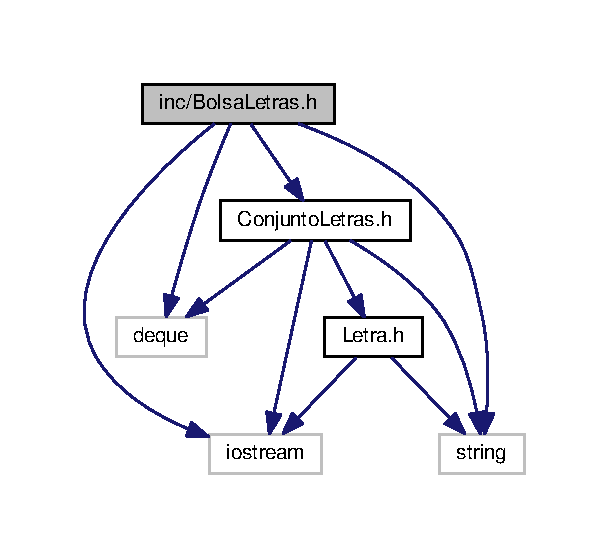
\includegraphics[width=292pt]{_bolsa_letras_8h__incl}
\end{center}
\end{figure}
Gráfico de los archivos que directa o indirectamente incluyen a este archivo\+:\nopagebreak
\begin{figure}[H]
\begin{center}
\leavevmode
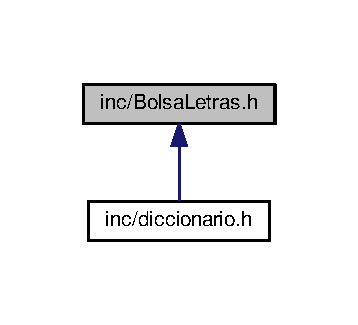
\includegraphics[width=172pt]{_bolsa_letras_8h__dep__incl}
\end{center}
\end{figure}
\subsection*{Clases}
\begin{DoxyCompactItemize}
\item 
class \hyperlink{class_bolsa_letras}{Bolsa\+Letras}
\begin{DoxyCompactList}\small\item\em T\+DA \hyperlink{class_bolsa_letras}{Bolsa\+Letras} {\bfseries Definición\+:} \hyperlink{class_bolsa_letras}{Bolsa\+Letras} guarda todos los caracteres que se pueden usar y obtiene las letras disponibles en el juego de forma aleatoria. \end{DoxyCompactList}\end{DoxyCompactItemize}


\subsection{Descripción detallada}
\begin{DoxyAuthor}{Autor}
Carlos Garcia Segura, Jose Maria Poblador Marquez 
\end{DoxyAuthor}

\hypertarget{_conjunto_letras_8h}{}\section{Referencia del Archivo inc/\+Conjunto\+Letras.h}
\label{_conjunto_letras_8h}\index{inc/\+Conjunto\+Letras.\+h@{inc/\+Conjunto\+Letras.\+h}}
{\ttfamily \#include $<$iostream$>$}\\*
{\ttfamily \#include $<$string$>$}\\*
{\ttfamily \#include \char`\"{}Letra.\+h\char`\"{}}\\*
{\ttfamily \#include $<$deque$>$}\\*
Dependencia gráfica adjunta para Conjunto\+Letras.\+h\+:\nopagebreak
\begin{figure}[H]
\begin{center}
\leavevmode
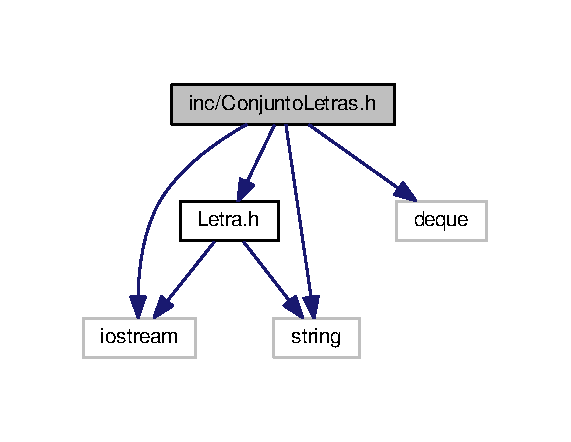
\includegraphics[width=274pt]{_conjunto_letras_8h__incl}
\end{center}
\end{figure}
Gráfico de los archivos que directa o indirectamente incluyen a este archivo\+:\nopagebreak
\begin{figure}[H]
\begin{center}
\leavevmode
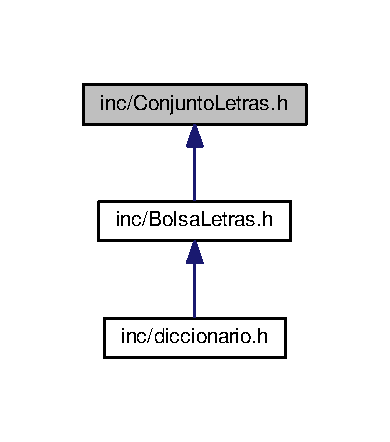
\includegraphics[width=187pt]{_conjunto_letras_8h__dep__incl}
\end{center}
\end{figure}
\subsection*{Clases}
\begin{DoxyCompactItemize}
\item 
class \hyperlink{class_conjunto_letras}{Conjunto\+Letras}
\begin{DoxyCompactList}\small\item\em T\+DA \hyperlink{_conjunto_letras_8h}{Conjunto\+Letras.\+h} {\bfseries Definición\+:} La clase conjunto letras guarda un conjunto de Letras. \end{DoxyCompactList}\end{DoxyCompactItemize}


\subsection{Descripción detallada}
\begin{DoxyAuthor}{Autor}
Carlos Garcia Segura, Jose Maria Poblador Marquez 
\end{DoxyAuthor}

\hypertarget{diccionario_8h}{}\section{Referencia del Archivo inc/diccionario.h}
\label{diccionario_8h}\index{inc/diccionario.\+h@{inc/diccionario.\+h}}
{\ttfamily \#include $<$vector$>$}\\*
{\ttfamily \#include $<$string$>$}\\*
{\ttfamily \#include \char`\"{}Arbol\+General.\+h\char`\"{}}\\*
{\ttfamily \#include \char`\"{}Bolsa\+Letras.\+h\char`\"{}}\\*
{\ttfamily \#include \char`\"{}Letra.\+h\char`\"{}}\\*
Dependencia gráfica adjunta para diccionario.\+h\+:\nopagebreak
\begin{figure}[H]
\begin{center}
\leavevmode
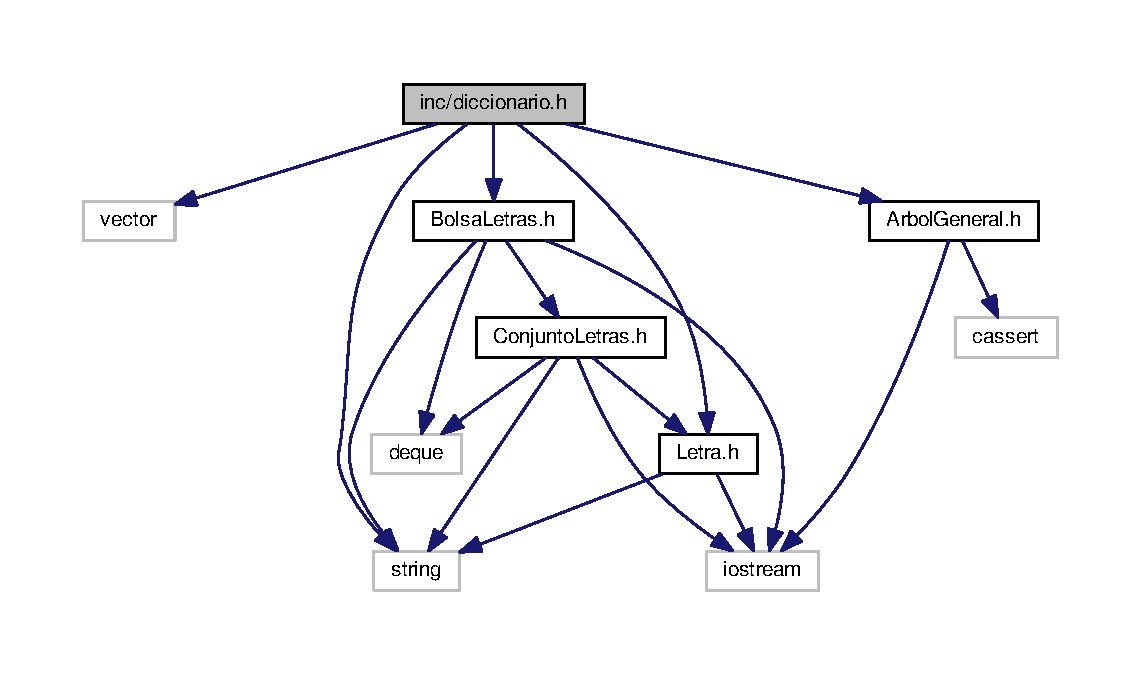
\includegraphics[width=350pt]{diccionario_8h__incl}
\end{center}
\end{figure}
\subsection*{Clases}
\begin{DoxyCompactItemize}
\item 
class \hyperlink{class_diccionario}{Diccionario}
\begin{DoxyCompactList}\small\item\em Clase \hyperlink{class_diccionario}{Diccionario} {\bfseries Definición\+:} La clase diccionario contiene un arbol general en el que se guardan las letras formando palabras. \end{DoxyCompactList}\item 
class \hyperlink{class_diccionario_1_1iterator}{Diccionario\+::iterator}
\begin{DoxyCompactList}\small\item\em Iterador del diccionario. \end{DoxyCompactList}\end{DoxyCompactItemize}


\subsection{Descripción detallada}
\begin{DoxyAuthor}{Autor}
Carlos Garcia Segura, Jose Maria Poblador Marquez 
\end{DoxyAuthor}

\hypertarget{_letra_8h}{}\section{Referencia del Archivo inc/\+Letra.h}
\label{_letra_8h}\index{inc/\+Letra.\+h@{inc/\+Letra.\+h}}
{\ttfamily \#include $<$iostream$>$}\\*
{\ttfamily \#include $<$string$>$}\\*
Dependencia gráfica adjunta para Letra.\+h\+:\nopagebreak
\begin{figure}[H]
\begin{center}
\leavevmode
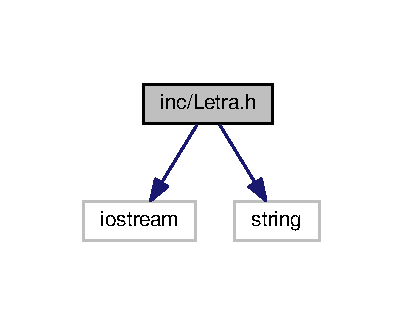
\includegraphics[width=194pt]{_letra_8h__incl}
\end{center}
\end{figure}
Gráfico de los archivos que directa o indirectamente incluyen a este archivo\+:\nopagebreak
\begin{figure}[H]
\begin{center}
\leavevmode
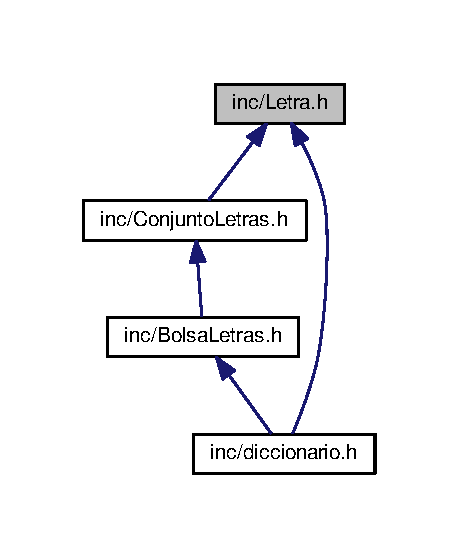
\includegraphics[width=220pt]{_letra_8h__dep__incl}
\end{center}
\end{figure}
\subsection*{Clases}
\begin{DoxyCompactItemize}
\item 
class \hyperlink{class_letra}{Letra}
\begin{DoxyCompactList}\small\item\em T\+DA \hyperlink{class_letra}{Letra} {\bfseries Definición\+:} La clase letra guarda la informacion sobre cada letra. \end{DoxyCompactList}\end{DoxyCompactItemize}


\subsection{Descripción detallada}
\begin{DoxyAuthor}{Autor}
Carlos Garcia Segura, Jose Maria Poblador Marquez 
\end{DoxyAuthor}

%--- End generated contents ---

% Index
\backmatter
\newpage
\phantomsection
\clearemptydoublepage
\addcontentsline{toc}{chapter}{Índice}
\printindex

\end{document}
